
% LaTeX Beamer file automatically generated from DocOnce
% https://github.com/doconce/doconce

%-------------------- begin beamer-specific preamble ----------------------

\documentclass{beamer}

\usetheme{red_plain}
\usecolortheme{default}

% turn off the almost invisible, yet disturbing, navigation symbols:
\setbeamertemplate{navigation symbols}{}

% Examples on customization:
%\usecolortheme[named=RawSienna]{structure}
%\usetheme[height=7mm]{Rochester}
%\setbeamerfont{frametitle}{family=\rmfamily,shape=\itshape}
%\setbeamertemplate{items}[ball]
%\setbeamertemplate{blocks}[rounded][shadow=true]
%\useoutertheme{infolines}
%
%\usefonttheme{}
%\useinntertheme{}
%
%\setbeameroption{show notes}
%\setbeameroption{show notes on second screen=right}

% fine for B/W printing:
%\usecolortheme{seahorse}

\usepackage{pgf}
\usepackage{graphicx}
\usepackage{epsfig}
\usepackage{relsize}

\usepackage{fancybox}  % make sure fancybox is loaded before fancyvrb

\usepackage{fancyvrb}
\usepackage{minted} % requires pygments and latex -shell-escape filename
%\usepackage{anslistings}
%\usepackage{listingsutf8}

\usepackage{amsmath,amssymb,bm}
%\usepackage[latin1]{inputenc}
\usepackage[T1]{fontenc}
\usepackage[utf8]{inputenc}
\usepackage{colortbl}
\usepackage[english]{babel}
\usepackage{tikz}
\usepackage{framed}
% Use some nice templates
\beamertemplatetransparentcovereddynamic

% --- begin table of contents based on sections ---
% Delete this, if you do not want the table of contents to pop up at
% the beginning of each section:
% (Only section headings can enter the table of contents in Beamer
% slides generated from DocOnce source, while subsections are used
% for the title in ordinary slides.)
\AtBeginSection[]
{
  \begin{frame}<beamer>[plain]
  \frametitle{}
  %\frametitle{Outline}
  \tableofcontents[currentsection]
  \end{frame}
}
% --- end table of contents based on sections ---

% If you wish to uncover everything in a step-wise fashion, uncomment
% the following command:

%\beamerdefaultoverlayspecification{<+->}

\newcommand{\shortinlinecomment}[3]{\note{\textbf{#1}: #2}}
\newcommand{\longinlinecomment}[3]{\shortinlinecomment{#1}{#2}{#3}}

\definecolor{linkcolor}{rgb}{0,0,0.4}
\hypersetup{
    colorlinks=true,
    linkcolor=linkcolor,
    urlcolor=linkcolor,
    pdfmenubar=true,
    pdftoolbar=true,
    bookmarksdepth=3
    }
\setlength{\parskip}{0pt}  % {1em}

\newenvironment{doconceexercise}{}{}
\newcounter{doconceexercisecounter}
\newenvironment{doconce:movie}{}{}
\newcounter{doconce:movie:counter}

\newcommand{\subex}[1]{\noindent\textbf{#1}}  % for subexercises: a), b), etc

%-------------------- end beamer-specific preamble ----------------------

% Add user's preamble




% insert custom LaTeX commands...

\raggedbottom
\makeindex

%-------------------- end preamble ----------------------

\begin{document}

% matching end for #ifdef PREAMBLE

\newcommand{\exercisesection}[1]{\subsection*{#1}}



% ------------------- main content ----------------------



% ----------------- title -------------------------

\title{Using Machine Learning to Classify Phase Transitions}

% ----------------- author(s) -------------------------

\author{Morten Hjorth-Jensen\inst{1}}
\institute{Department of Physics and Center for Computing in Science Education, University of Oslo, Norway\inst{1}}
% ----------------- end author(s) -------------------------

\date{CEACM Flagship School: Machine Learning in Physical Sciences: Theory and Applications
% <optional titlepage figure>
% <optional copyright>
}

May 26, 2025 - May 30, 2025

\begin{frame}[plain,fragile]
\titlepage
\end{frame}

\begin{frame}[plain,fragile]
\frametitle{What is this about?}

\begin{block}{}
These notes, with pertinent exercises cover the following topics. All the material here can be found in the PDF files, codes and jupyter-notebooks at the above \textbf{doc} folder, see the \textbf{pub} subfolder, link to be added  
\begin{enumerate}
\item Phase Transitions {\&} Critical Phenomena: Definitions and key concepts (order parameters, critical points, first vs second order).

\item Spin Models: 2D Ising model and the q-state Potts model (examples of phase transitions).

\item Data Generation: Monte Carlo simulations for sampling spin configurations across temperatures.

\item Unsupervised Learning (PCA): Principal Component Analysis to visualize phase separation without labels.

\item Supervised Learning (CNN): Convolutional Neural Networks for classifying phases from raw configurations.

\item Generative Models (VAE): Variational Autoencoders for latent representation learning and critical anomaly detection.

\item Comparisons: Interpretability and performance trade-offs between PCA, CNN, and VAE.
\end{enumerate}

\noindent
\end{block}
\end{frame}

\begin{frame}[plain,fragile]
\frametitle{AI/ML and some statements you may have heard (and what do they mean?)}

\begin{enumerate}
\item Fei-Fei Li on ImageNet: \textbf{map out the entire world of objects} (\href{{https://cacm.acm.org/news/219702-the-data-that-transformed-ai-research-and-possibly-the-world/fulltext}}{The data that transformed AI research})

\item Russell and Norvig in their popular textbook: \textbf{relevant to any intellectual task; it is truly a universal field} (\href{{http://aima.cs.berkeley.edu/}}{Artificial Intelligence, A modern approach})

\item Woody Bledsoe puts it more bluntly: \textbf{in the long run, AI is the only science} (quoted in Pamilla McCorduck, \href{{https://www.pamelamccorduck.com/machines-who-think}}{Machines who think})
\end{enumerate}

\noindent
If you wish to have a critical read on AI/ML from a societal point of view, see \href{{https://www.katecrawford.net/}}{Kate Crawford's recent text Atlas of AI}. 

\textbf{Here: with AI/ML we intend a collection of machine learning methods with an emphasis on statistical learning and data analysis}
\end{frame}

\begin{frame}[plain,fragile]
\frametitle{Types of machine learning}

\begin{block}{}
The approaches to machine learning are many, but are often split into two main categories. 
In \emph{supervised learning} we know the answer to a problem,
and let the computer deduce the logic behind it. On the other hand, \emph{unsupervised learning}
is a method for finding patterns and relationship in data sets without any prior knowledge of the system.

An important  third category is  \emph{reinforcement learning}. This is a paradigm 
of learning inspired by behavioural psychology, where learning is achieved by trial-and-error, 
solely from rewards and punishment.
\end{block}
\end{frame}

\begin{frame}[plain,fragile]
\frametitle{Main categories}

\begin{block}{}
Another way to categorize machine learning tasks is to consider the desired output of a system.
Some of the most common tasks are:

\begin{itemize}
  \item Classification: Outputs are divided into two or more classes. The goal is to   produce a model that assigns inputs into one of these classes. An example is to identify  digits based on pictures of hand-written ones. Classification is typically supervised learning.

  \item Regression: Finding a functional relationship between an input data set and a reference data set.   The goal is to construct a function that maps input data to continuous output values.

  \item Clustering: Data are divided into groups with certain common traits, without knowing the different groups beforehand.  It is thus a form of unsupervised learning.
\end{itemize}

\noindent
\end{block}
\end{frame}

\begin{frame}[plain,fragile]
\frametitle{The plethora  of machine learning algorithms/methods}

\begin{enumerate}
\item Deep learning: Neural Networks (NN), Convolutional NN, Recurrent NN, Boltzmann machines, autoencoders and variational autoencoders  and generative adversarial networks, stable diffusion and many more generative models

\item Bayesian statistics and Bayesian Machine Learning, Bayesian experimental design, Bayesian Regression models, Bayesian neural networks, Gaussian processes and much more

\item Dimensionality reduction (Principal component analysis), Clustering Methods and more

\item Ensemble Methods, Random forests, bagging and voting methods, gradient boosting approaches 

\item Linear and logistic regression, Kernel methods, support vector machines and more

\item Reinforcement Learning; Transfer Learning and more 
\end{enumerate}

\noindent
\end{frame}

\begin{frame}[plain,fragile]
\frametitle{Example of generative modeling, \href{{https://www.oreilly.com/library/view/generative-deep-learning/9781098134174/ch01.html}}{taken from Generative Deep Learning by David Foster}}

\vspace{6mm}

% inline figure
\centerline{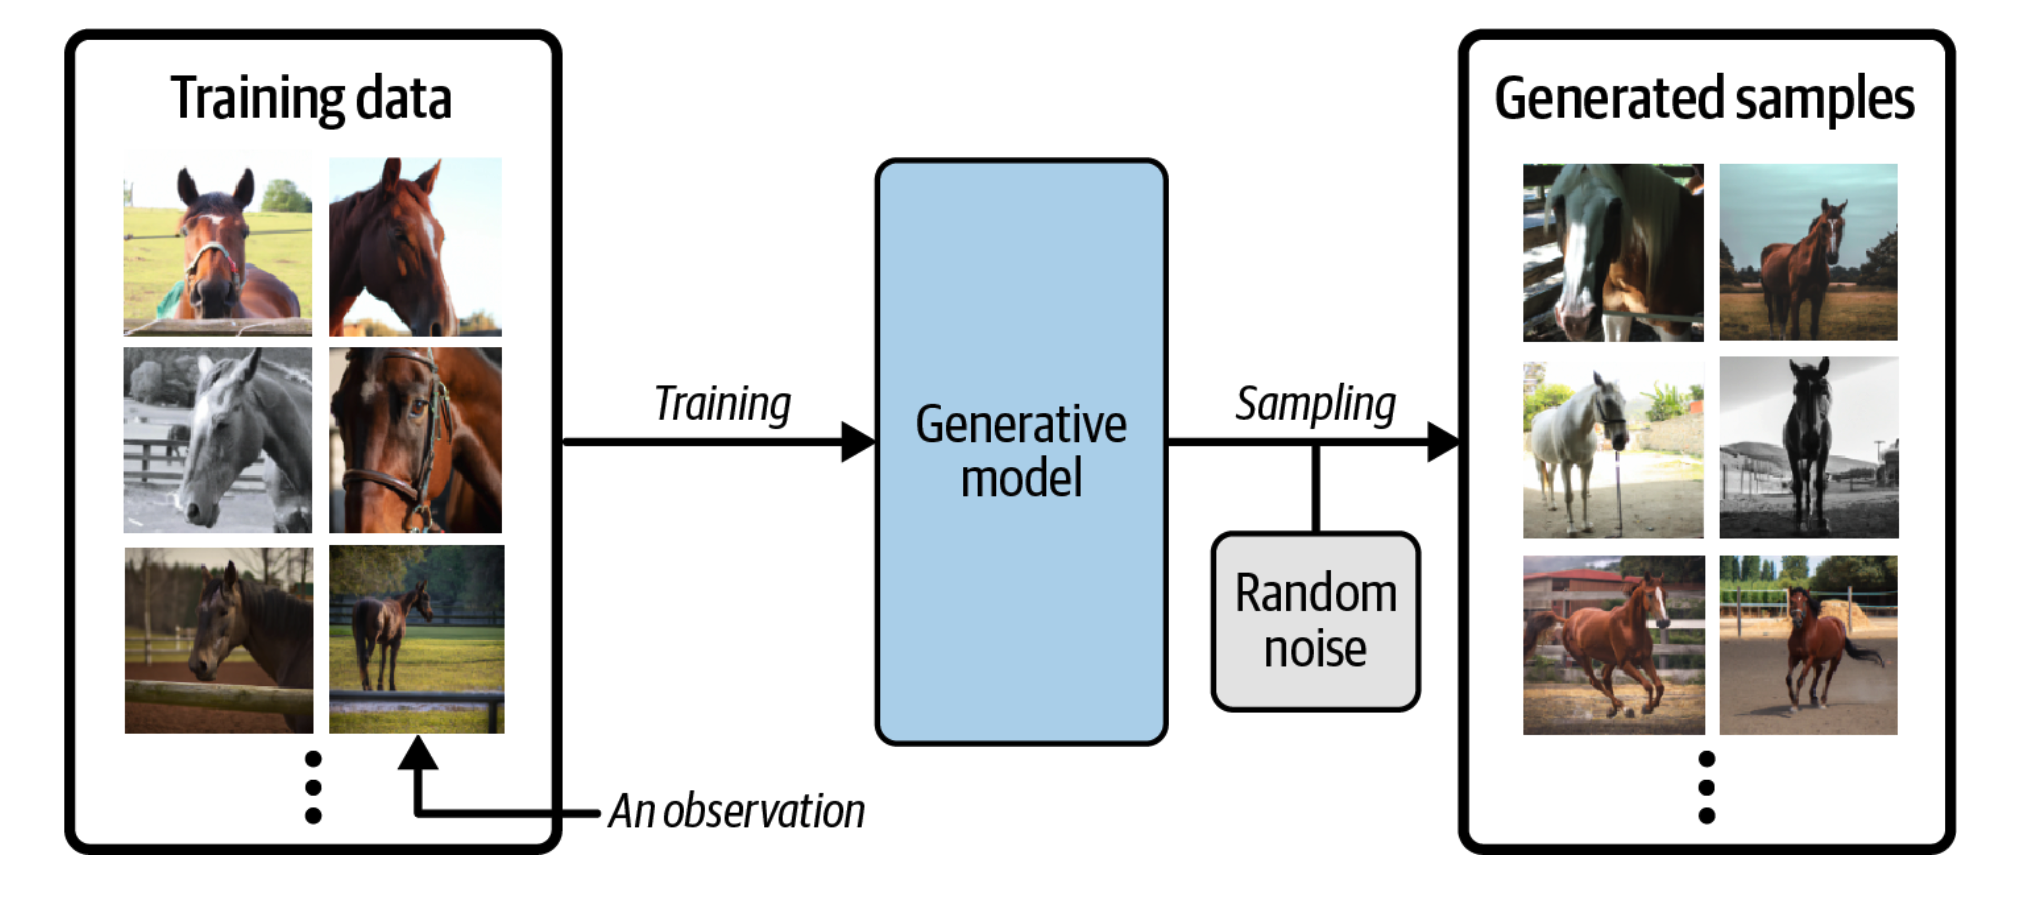
\includegraphics[width=1.0\linewidth]{figures/generativelearning.png}}

\vspace{6mm}
\end{frame}

\begin{frame}[plain,fragile]
\frametitle{Example of discriminative modeling, \href{{https://www.oreilly.com/library/view/generative-deep-learning/9781098134174/ch01.html}}{taken from Generative Deeep Learning by David Foster}}

\vspace{6mm}

% inline figure
\centerline{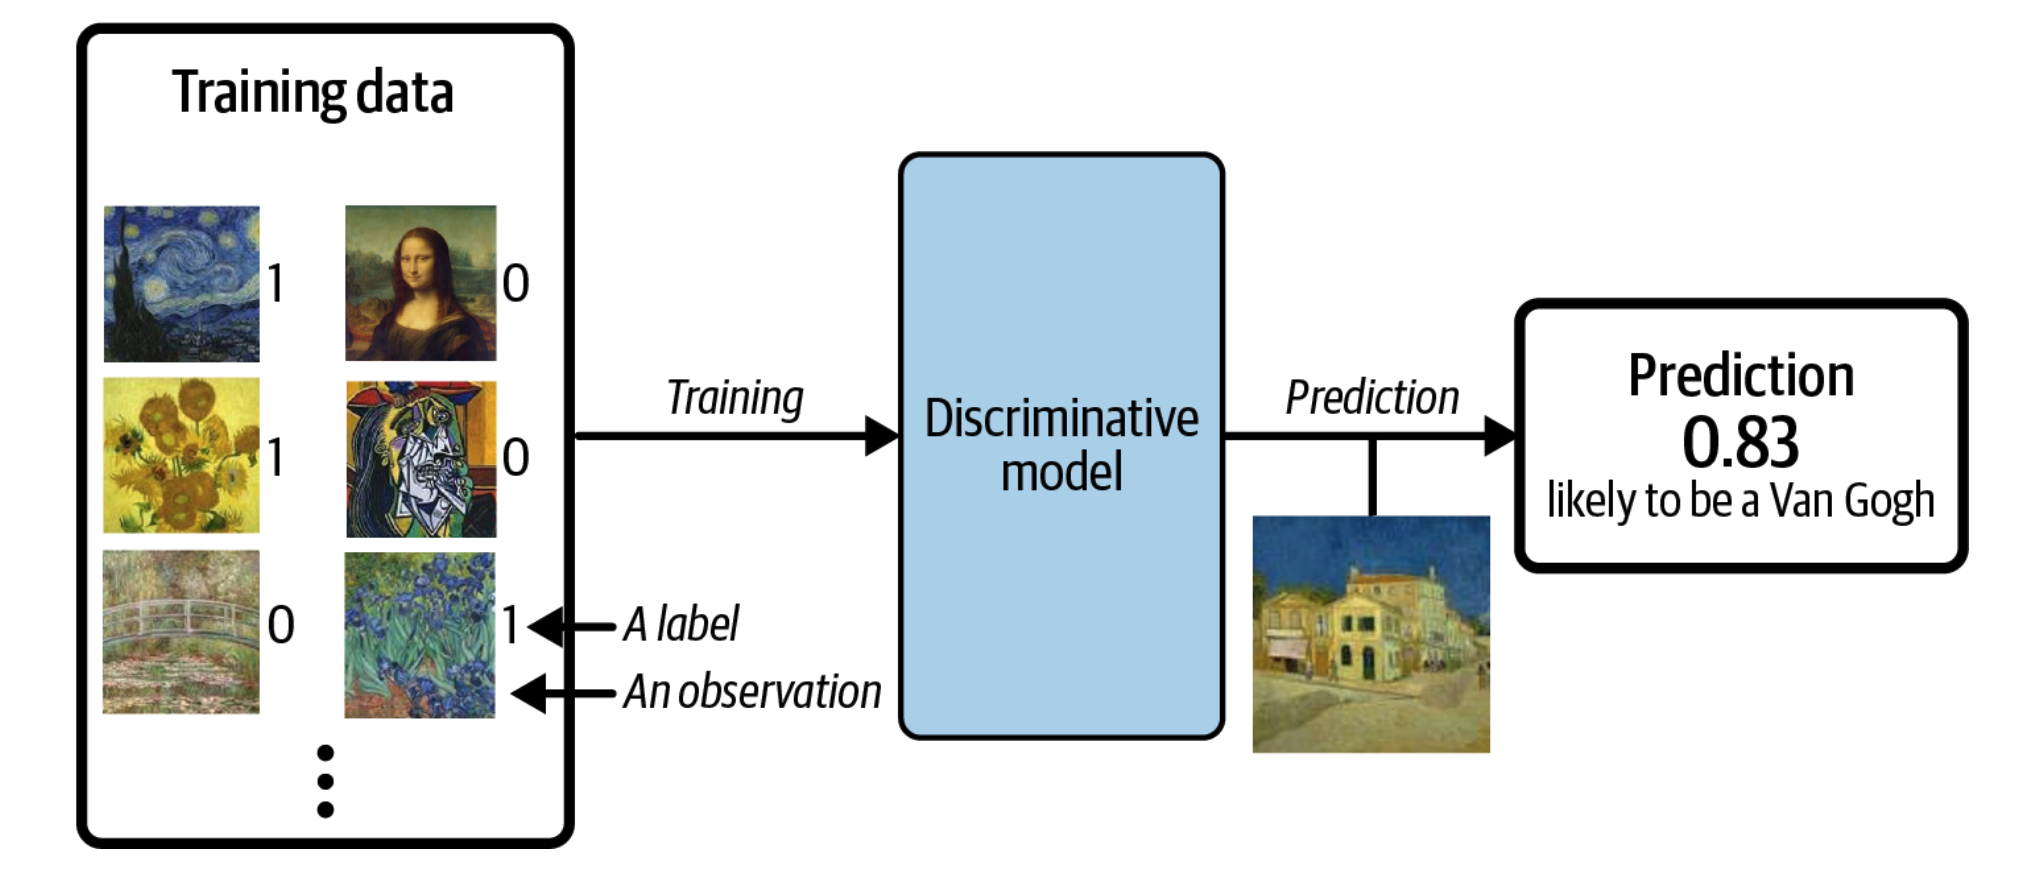
\includegraphics[width=1.0\linewidth]{figures/standarddeeplearning.png}}

\vspace{6mm}
\end{frame}

\begin{frame}[plain,fragile]
\frametitle{Taxonomy of generative deep learning, \href{{https://www.oreilly.com/library/view/generative-deep-learning/9781098134174/ch01.html}}{taken from Generative Deep Learning by David Foster}}

\vspace{6mm}

% inline figure
\centerline{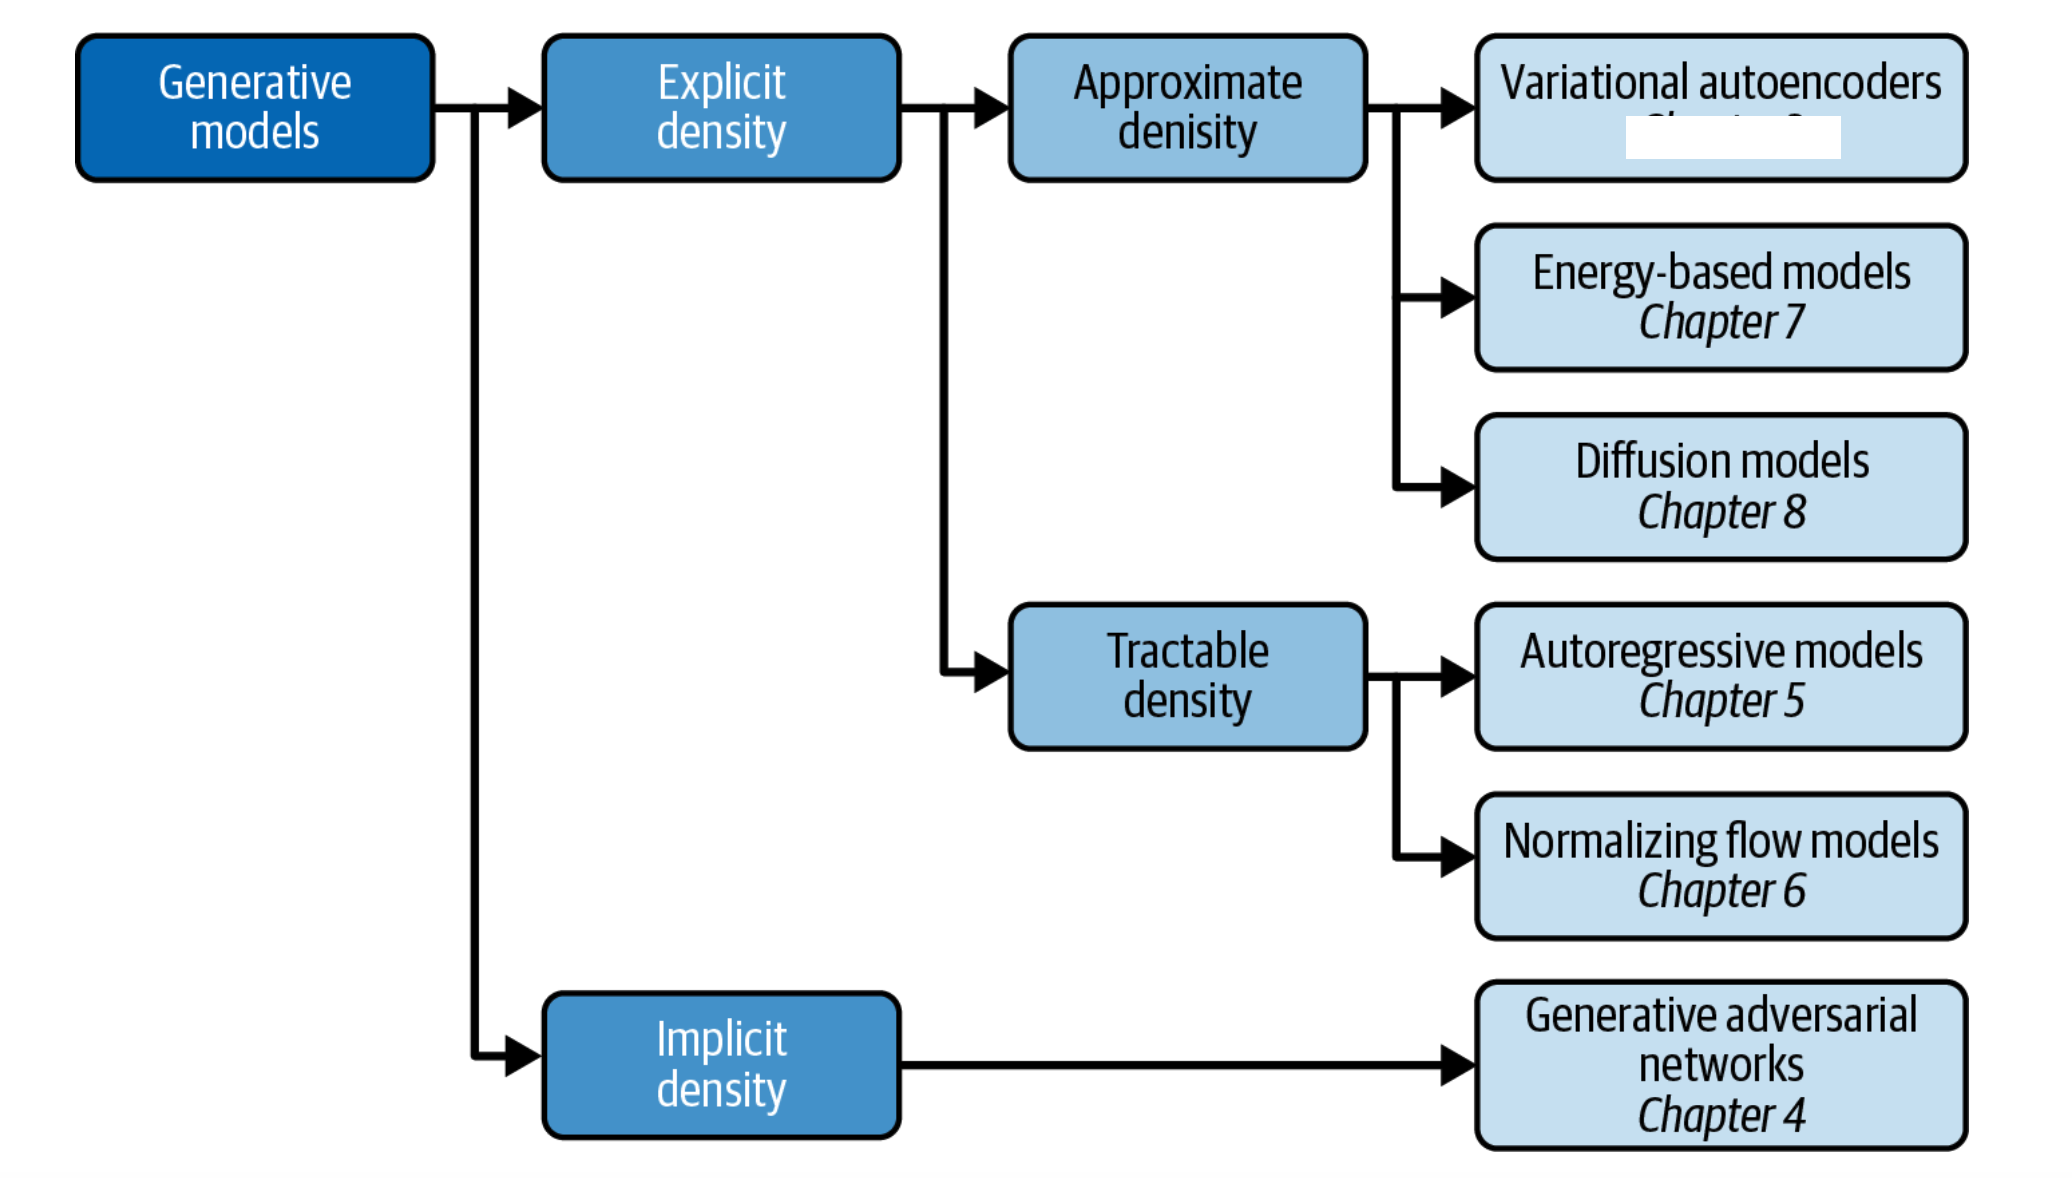
\includegraphics[width=1.0\linewidth]{figures/generativemodels.png}}

\vspace{6mm}
\end{frame}

\begin{frame}[plain,fragile]
\frametitle{Good books with hands-on material and codes}

\begin{block}{}
\begin{itemize}
\item \href{{https://sebastianraschka.com/blog/2022/ml-pytorch-book.html}}{Sebastian Rashcka et al, Machine learning with Sickit-Learn and PyTorch}

\item \href{{https://www.oreilly.com/library/view/generative-deep-learning/9781098134174/ch01.html}}{David Foster, Generative Deep Learning with TensorFlow}

\item \href{{https://github.com/PacktPublishing/Hands-On-Generative-AI-with-Python-and-TensorFlow-2}}{Bali and Gavras, Generative AI with Python and TensorFlow 2}
\end{itemize}

\noindent
\end{block}

All three books have GitHub addresses from where  one can download all codes. We will borrow most of the material from these three texts as well as 
from Goodfellow, Bengio and Courville's text \href{{https://www.deeplearningbook.org/}}{Deep Learning}
\end{frame}

\begin{frame}[plain,fragile]
\frametitle{What are the basic Machine Learning ingredients?}

\begin{block}{}
Almost every problem in ML and data science starts with the same ingredients:
\begin{itemize}
\item The dataset $\bm{x}$ (could be some observable quantity of the system we are studying)

\item A model which is a function of a set of parameters $\bm{\alpha}$ that relates to the dataset, say a likelihood  function $p(\bm{x}\vert \bm{\alpha})$ or just a simple model $f(\bm{\alpha})$

\item A so-called \textbf{loss/cost/risk} function $\mathcal{C} (\bm{x}, f(\bm{\alpha}))$ which allows us to decide how well our model represents the dataset. 
\end{itemize}

\noindent
We seek to minimize the function $\mathcal{C} (\bm{x}, f(\bm{\alpha}))$ by finding the parameter values which minimize $\mathcal{C}$. This leads to  various minimization algorithms. It may surprise many, but at the heart of all machine learning algortihms there is an optimization problem. 
\end{block}
\end{frame}

\begin{frame}[plain,fragile]
\frametitle{Low-level machine learning, the family of ordinary least squares methods}

Our data which we want to apply a machine learning method on, consist
of a set of inputs $\bm{x}^T=[x_0,x_1,x_2,\dots,x_{n-1}]$ and the
outputs we want to model $\bm{y}^T=[y_0,y_1,y_2,\dots,y_{n-1}]$.
We assume  that the output data can be represented (for a regression case) by a continuous function $f$
through
\[
\bm{y}=f(\bm{x})+\bm{\epsilon}.
\]
\end{frame}

\begin{frame}[plain,fragile]
\frametitle{Setting up the equations}

In linear regression we approximate the unknown function with another
continuous function $\tilde{\bm{y}}(\bm{x})$ which depends linearly on
some unknown parameters
$\bm{\theta}^T=[\theta_0,\theta_1,\theta_2,\dots,\theta_{p-1}]$.

The input data can be organized in terms of a so-called design matrix 
with an approximating function $\bm{\tilde{y}}$ 
\[
\bm{\tilde{y}}= \bm{X}\bm{\theta},
\]
\end{frame}

\begin{frame}[plain,fragile]
\frametitle{The objective/cost/loss function}

The  simplest approach is the mean squared error
\[
C(\bm{\Theta})=\frac{1}{n}\sum_{i=0}^{n-1}\left(y_i-\tilde{y}_i\right)^2=\frac{1}{n}\left\{\left(\bm{y}-\bm{\tilde{y}}\right)^T\left(\bm{y}-\bm{\tilde{y}}\right)\right\},
\]
or using the matrix $\bm{X}$ and in a more compact matrix-vector notation as
\[
C(\bm{\Theta})=\frac{1}{n}\left\{\left(\bm{y}-\bm{X}\bm{\theta}\right)^T\left(\bm{y}-\bm{X}\bm{\theta}\right)\right\}.
\]
This function represents one of many possible ways to define the so-called cost function.
\end{frame}

\begin{frame}[plain,fragile]
\frametitle{Training solution}

Optimizing with respect to the unknown parameters $\theta_j$ we get 
\[
\bm{X}^T\bm{y} = \bm{X}^T\bm{X}\bm{\theta},  
\]
and if the matrix $\bm{X}^T\bm{X}$ is invertible we have the optimal values
\[
\hat{\bm{\theta}} =\left(\bm{X}^T\bm{X}\right)^{-1}\bm{X}^T\bm{y}.
\]

We say we 'learn' the unknown parameters $\bm{\theta}$ from the last equation.
\end{frame}

\begin{frame}[plain,fragile]
\frametitle{Selected references}

\begin{block}{}
\begin{itemize}
\item \href{{https://arxiv.org/abs/1803.08823}}{Mehta et al.} and \href{{https://www.sciencedirect.com/science/article/pii/S0370157319300766?via%3Dihub}}{Physics Reports (2019)}.

\item \href{{https://link.aps.org/doi/10.1103/RevModPhys.91.045002}}{Machine Learning and the Physical Sciences by Carleo et al}

\item \href{{https://journals.aps.org/rmp/abstract/10.1103/RevModPhys.94.031003}}{Artificial Intelligence and Machine Learning in Nuclear Physics, Amber Boehnlein et al., Reviews Modern of Physics 94, 031003 (2022)} 

\item \href{{https://journals.aps.org/prresearch/pdf/10.1103/PhysRevResearch.5.033062}}{Dilute neutron star matter from neural-network quantum states by Fore et al, Physical Review Research 5, 033062 (2023)}

\item \href{{https://doi.org/10.48550/arXiv.2305.08831}}{Neural-network quantum states for ultra-cold Fermi gases, Jane Kim et al, Nature Physics Communcication, submitted}

\item \href{{https://doi.org/10.48550/arXiv.2305.07240}}{Message-Passing Neural Quantum States for the Homogeneous Electron Gas, Gabriel Pescia, Jane Kim et al.~arXiv.2305.07240,}

\item "Efficient solutions of fermionic systems using artificial neural networks, Nordhagen et al, Frontiers in Physics
\end{itemize}

\noindent
\end{block}
\end{frame}

\begin{frame}[plain,fragile]
\frametitle{Machine learning. A simple perspective on the interface between ML and Physics}

\vspace{6mm}

% inline figure
\centerline{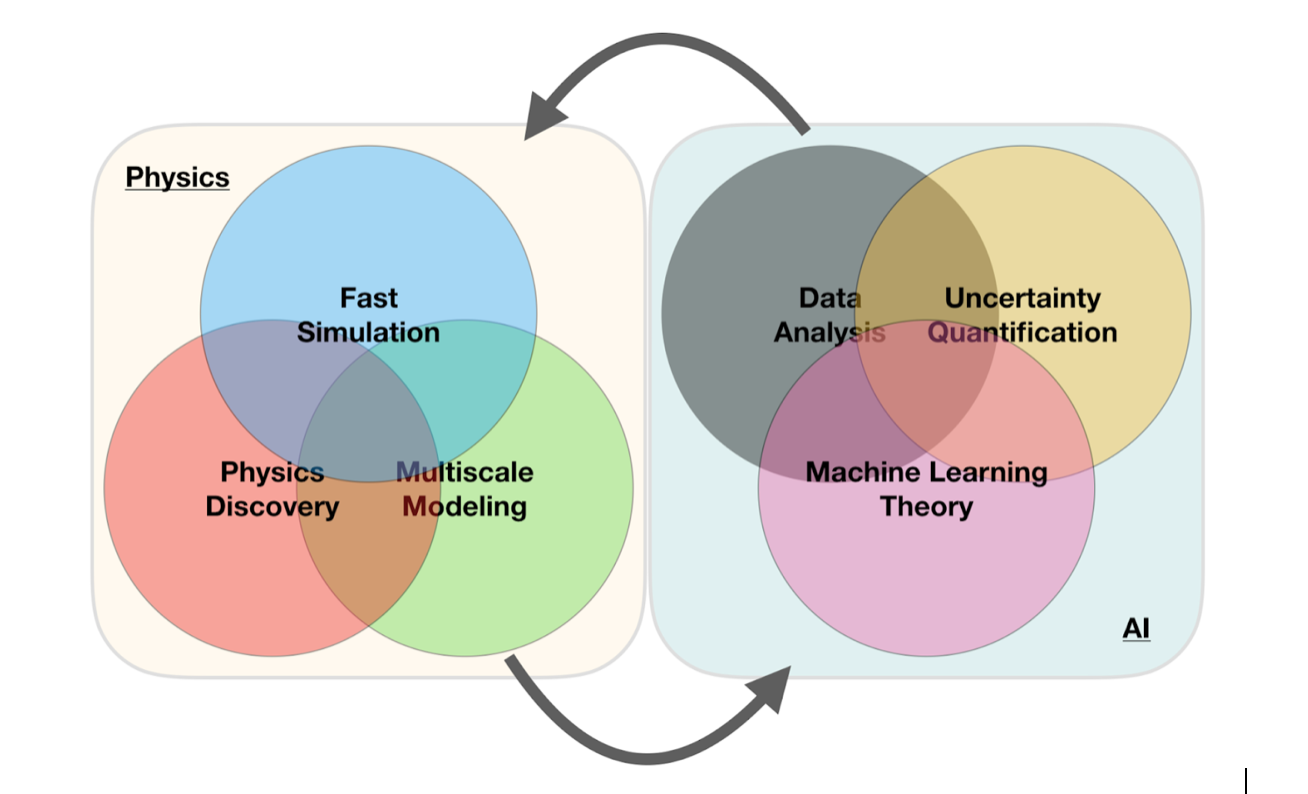
\includegraphics[width=1.0\linewidth]{figures/mlimage.png}}

\vspace{6mm}
\end{frame}

\begin{frame}[plain,fragile]
\frametitle{ML in Nuclear  Physics (or any field in physics)}

\vspace{6mm}

% inline figure
\centerline{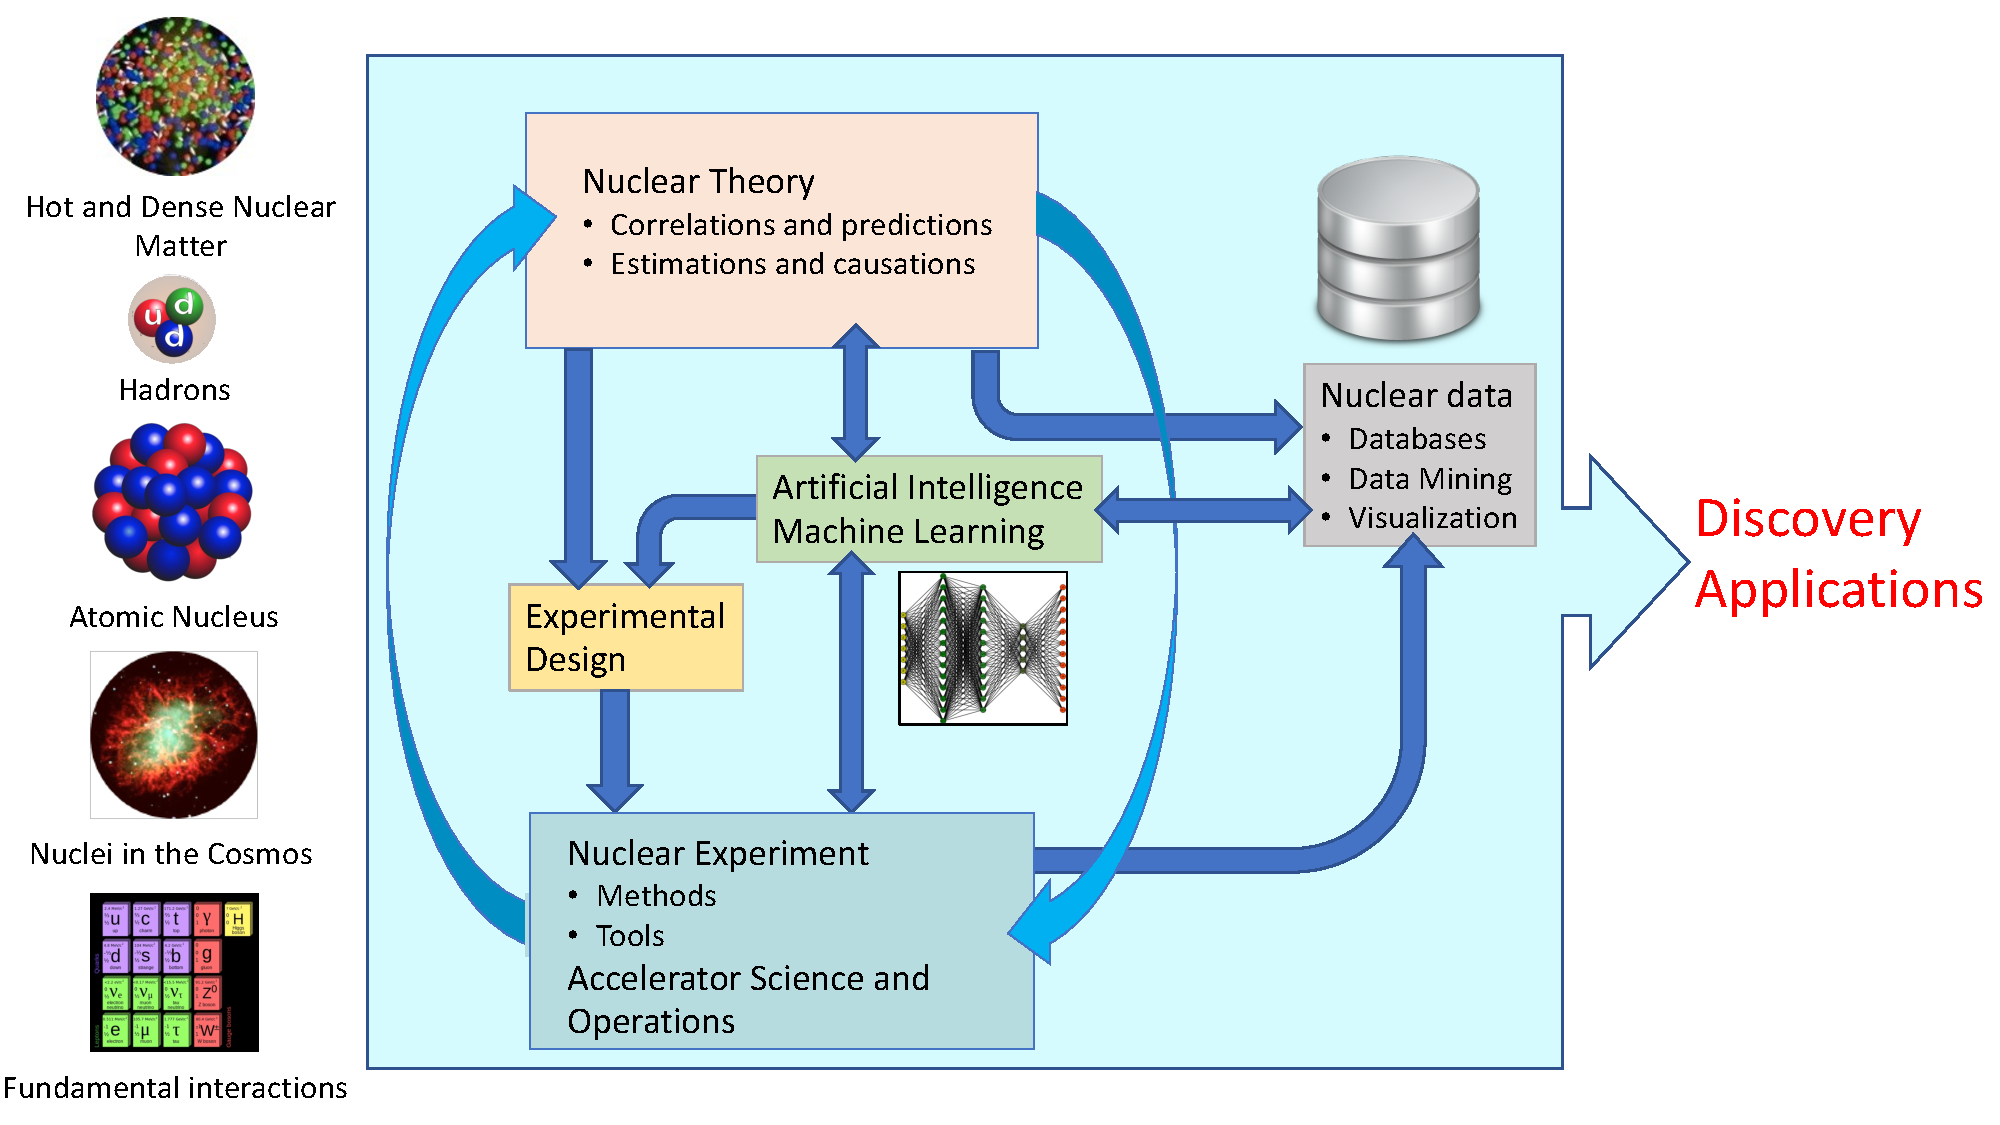
\includegraphics[width=1.0\linewidth]{figures/ML-NP.pdf}}

\vspace{6mm}
\end{frame}

\begin{frame}[plain,fragile]
\frametitle{Phase Transitions and Critical Phenomena}

\begin{enumerate}
\item Definition: A phase transition is characterized by an abrupt, non-analytic change in a macroscopic property of a system as some external parameter (e.g.~temperature) is varied . In simpler terms, the system’s state or phase changes dramatically at a critical point.

\item Order Parameter: Associated with each phase transition is an order parameter – a quantity that is zero in one phase and non-zero in the other. For example, magnetization plays the role of an order parameter in magnetic systems, distinguishing ordered (magnetized) from disordered (unmagnetized) phases.

\item Critical Point: At the critical temperature (or pressure, etc.), the order parameter changes (continuous or discontinuous) and the system exhibits critical phenomena: large fluctuations, divergence of correlation length, and the onset of scale invariance. Critical points of second-order transitions feature continuous change of the order parameter with characteristic critical exponents and universal behavior across different systems.
\end{enumerate}

\noindent
\end{frame}

\begin{frame}[plain,fragile]
\frametitle{Phase Transitions: Definitions}

\begin{enumerate}
\item A \emph{phase transition} is a qualitative change in the state of a system when a control parameter (e.g.\ temperature) passes a critical point.

\item \textbf{Order parameter}: quantity that distinguishes phases (e.g.\ magnetization $M$ for magnetic systems).

\item \textbf{Order vs disorder}: e.g.\ below $T_c$ a ferromagnet has $|M|>0$ (ordered), above $T_c$ $M=0$ (disordered).

\item Phases can break symmetries; transitions can be \emph{continuous} (second-order) or \emph{first-order}.
\end{enumerate}

\noindent
\end{frame}

\begin{frame}[plain,fragile]
\frametitle{Order Parameter and Symmetry Breaking}

\begin{enumerate}
\item Phase transitions often involve spontaneous symmetry breaking (e.g.\ Ising model $Z_2$ symmetry).

\item The order parameter (e.g.\ magnetization $M = \frac{1}{N}\sum_i s_i$) changes behavior at $T_c$.

\item In ferromagnets: $M=0$ for $T>T_c$ (symmetric paramagnet), $M\neq 0$ for $T<T_c$ (broken symmetry).

\item Example: in 2D Ising model, two symmetric ordered states (up/down) below $T_c$.
\end{enumerate}

\noindent
\end{frame}

\begin{frame}[plain,fragile]
\frametitle{Critical Phenomena and Scaling}

\begin{enumerate}
\item Near a continuous transition, observables follow power laws: $M \sim |T-T_c|^\beta$, correlation length $\xi \sim |T-T_c|^{-\nu}$, etc.

\item \textbf{Critical exponents} ($\alpha,\beta,\gamma,\nu,\dots$) characterize singular behavior.

\item Universality: systems with the same symmetry and dimension share exponents.

\item The classical example is the  two-dimensional  Ising exponents known analytically (Onsager).

\item At $T\to T_c$, correlation length $\xi\to\infty$, large-scale fluctuations appear.
\end{enumerate}

\noindent
\end{frame}

\begin{frame}[plain,fragile]
\frametitle{2D Ising Model: Definition}

\begin{enumerate}
\item Spins $s_i = \pm 1$ on a 2D square lattice, nearest-neighbor ferromagnetic coupling.

\item Hamiltonian: $H = -J \sum_{\langle i,j\rangle} s_i s_j,$ with $J>0$ favoring alignment.

\item Exhibits a second-order phase transition at critical temperature $T_c$.

\item Order parameter: magnetization $M = \frac{1}{N}\sum_i s_i$.

\item Below $T_c$, $M\neq0$ (ferromagnetic order); above $T_c$, $M=0$ (paramagnet).
\end{enumerate}

\noindent
\end{frame}

\begin{frame}[plain,fragile]
\frametitle{2D Ising Model: Critical Temperature}

\begin{enumerate}
\item Exact result (Onsager): critical point $T_c$ satisfies $T_c \approx \frac{2J}{\ln(1+\sqrt{2})}\approx 2.269J$.

\item At $T>T_c$: spins are mostly disordered, no net magnetization.

\item At $T<T_c$: long-range order develops (nonzero $M$).

\item Correlation length $\xi$ diverges at $T_c$ 

\item Example: at $T=T_c$ large clusters of aligned spins appear.
\end{enumerate}

\noindent
\end{frame}

\begin{frame}[plain,fragile]
\frametitle{q-State Potts Model: Definition}

\begin{itemize}
\item Generalization of Ising: each spin $s_i \in \{1,2,\dots,q\}$.

\item Ferromagnetic Potts Hamiltonian:
\end{itemize}

\noindent
     \[
       H = -J \sum_{\langle i,j\rangle} \delta_{s_i,s_j},
     \]
where $\delta_{a,b}=1$ if $a=b$, else $0$.
\begin{itemize}
\item If $q=2$, reduces to the Ising model. Higher $q$ allows richer symmetry breaking ($\mathbb{Z}_q$).

\item Widely used to study phase transitions with multiple equivalent ordered states.
\end{itemize}

\noindent
\end{frame}

\begin{frame}[plain,fragile]
\frametitle{2D Potts Model: Phase Behavior}

\begin{itemize}
\item In 2D, the ferromagnetic Potts model has a phase transition for all $q\ge1$ 

\item Exact critical point:
\end{itemize}

\noindent
     \[
       \frac{J}{k_B T_c} = \ln\!\bigl(1+\sqrt{q}\bigr).
     \]
\begin{itemize}
\item The nature of the transition depends on $q$ 
\begin{itemize}

  \item $1 \le q \le 4$: continuous (second-order) transition.

  \item $q > 4$: discontinuous (first-order) transition (latent heat appears).

\end{itemize}

\noindent
\item Example: $q=3,4$ have continuous transitions; $q=5$ and higher show first-order behavior.
\end{itemize}

\noindent
\end{frame}

\begin{frame}[plain,fragile]
\frametitle{Monte Carlo Sampling of Spin Models}

\begin{enumerate}
\item Use Monte Carlo (MC) to generate spin configurations at given $T$: sample from Boltzmann distribution $P\propto e^{-H/T}$.

\item Metropolis algorithm: attempt random single-spin flips to equilibrate the system.

\item Provides training data: spin configurations $\{s_i\}$ labeled by temperature or phase.

\item Ensures statistical equilibrium and detailed balance 

\item Efficient sampling (especially near $T_c$ cluster algorithms help, e.g.\ Wolff or Swendsen-Wang).
\end{enumerate}

\noindent
\end{frame}

\begin{frame}[plain,fragile]
\frametitle{Metropolis Algorithm}

\begin{itemize}
\item Initialize spins randomly or in a fixed state.

\item Repeat for many steps:
\begin{enumerate}

 \item Pick a random lattice site $i$.

 \item Propose flipping $s_i \to -s_i$ (Ising) or change state (Potts).

 \item Compute energy change $\Delta E$.

 \item If $\Delta E \le 0$, accept the flip (lower energy).

 \item Else accept with probability $\exp(-\Delta E/T)$ (Boltzmann factor) 

 \item Otherwise, reject and keep the old state.

\end{enumerate}

\noindent
\item After equilibration, record configurations as samples.
\end{itemize}

\noindent
\end{frame}

\begin{frame}[plain,fragile]
\frametitle{Metropolis Algorithm (Pseudo-code)}

\begin{minted}[fontsize=\fontsize{9pt}{9pt},linenos=false,mathescape,baselinestretch=1.0,fontfamily=tt,xleftmargin=2mm]{python}
for T in temperature_list:
   # Initialize lattice (e.g., random spins)
   config = random_configuration(Lx, Ly)
   for step in range(num_steps):
       i,j = random_site()
       dE = compute_deltaE(config, i, j)  # energy change if spin flipped
       if dE <= 0 or rand() < exp(-dE/T):
           flip_spin(config, i, j)
   record_configuration(config, T)

\end{minted}
\end{frame}

\begin{frame}[plain,fragile]
\frametitle{Monte Carlo Data for ML}

\begin{enumerate}
\item Generate many spin configurations across a range of temperatures $T$.

\item Label each configuration by its temperature or by phase (ordered/disordered).

\item This labeled dataset is used for \emph{supervised} methods (e.g.\ CNN).

\item For \emph{unsupervised} methods (PCA, VAE), labels are not used in training.

\item Data augmentation: one can use symmetries (e.g.\ spin flip) to enlarge dataset.
\end{enumerate}

\noindent
\end{frame}

\begin{frame}[plain,fragile]
\frametitle{Principal Component Analysis (PCA) Basics}

\begin{enumerate}
\item PCA is an unsupervised method for dimensionality reduction.

\item Finds orthogonal directions (principal components) of maximum variance in data.

\item Project data onto the first few PCs to visualize structure.

\item Advantages: linear, fast, and interpretable (PCs are linear combinations of features).

\item Disadvantage: only captures linear correlations (may miss complex features).
\end{enumerate}

\noindent
\end{frame}

\begin{frame}[plain,fragile]
\frametitle{PCA for Phase Identification}

\begin{enumerate}
\item Apply PCA to the ensemble of spin configurations (flattened to vectors).

\item The first principal component (PC1) often correlates with the order parameter (e.g.\ magnetization).

\item Hu et al. (2017) found PCA distinguishes different phases and can locate critical points 

\item By plotting data in the subspace of PCs, one sees separation of low-$T$ (ordered) vs high-$T$ (disordered) points.

\item No labels needed: phase transitions are revealed by clustering in PC space 
\end{enumerate}

\noindent
\end{frame}

\begin{frame}[plain,fragile]
\frametitle{PCA Workflow for Spin Data}

\begin{enumerate}
\item Collect data matrix $X$ of shape (num\_samples) $\times$ (num\_features), e.g.~$N\times (L\times L)$.

\item Subtract the mean from each column (feature) of $X$.

\item Compute covariance matrix $C = X^T X$ (or use SVD on $X$ directly).

\item Obtain eigenvalues/vectors of $C$: $C = U \Lambda U^T$. Columns of $U$ are principal directions.

\item Sort by eigenvalues (variance). Project $X$ onto top $k$ PCs: $X_{\rm red} = X\,U[:,1:k]$.

\item Analyze $X_{\rm red}$: e.g.~scatter plot PC1 vs PC2.
\end{enumerate}

\noindent
\end{frame}

\begin{frame}[plain,fragile]
\frametitle{PCA Example: Ising Model}

\begin{enumerate}
\item In the 2D Ising model, PC1 is essentially proportional to the overall magnetization.

\item At $T<T_c$, configurations cluster with large positive or negative PC1 (ordered states).

\item At $T>T_c$, configurations cluster near $PC1 \approx 0$ (disordered).

\item The variance captured by PC1 drops sharply at $T_c$, signaling the transition.

\item PCA automatically finds these features, without knowing the physics a priori.
\end{enumerate}

\noindent
\end{frame}

\begin{frame}[plain,fragile]
\frametitle{PCA Limitations}

\begin{enumerate}
\item PCA is linear: complex nonlinear features (e.g.\ vortex order) may not be captured.

\item Example: In a frustrated 2D spin model, PCA failed to detect certain correlations (vorticity) 

\item PCA does not directly classify; it provides features for clustering or visualization.

\item Sensitive to scaling: data should be normalized appropriately.

\item Still useful as a first-pass: identifies the most significant variations 
\end{enumerate}

\noindent
\end{frame}

\begin{frame}[plain,fragile]
\frametitle{PCA with PyTorch (Example Code)}

\begin{minted}[fontsize=\fontsize{9pt}{9pt},linenos=false,mathescape,baselinestretch=1.0,fontfamily=tt,xleftmargin=2mm]{python}
import torch

# X: tensor of shape (N, L*L) containing spin configurations as floats (e.g. +1/-1)
# Center the data
X = X - X.mean(dim=0, keepdim=True)

# Compute covariance (or use torch.pca_lowrank)
cov = torch.mm(X.t(), X) / (X.size(0)-1)

# Eigen-decomposition (SVD) of covariance
U, S, V = torch.svd(cov)

# Select first k principal components
k = 2
PCs = U[:, :k]  # shape (L*L, k)

# Project data onto principal components
X_reduced = torch.mm(X, PCs)  # shape (N, k)

\end{minted}
\end{frame}

\begin{frame}[plain,fragile]
\frametitle{Convolutional Neural Networks (CNNs)}

\begin{enumerate}
\item CNNs are deep neural networks designed for spatial data (e.g.~images).

\item Architecture: convolutional layers (feature detectors) + pooling, followed by fully connected layers.

\item In physics: treat spin lattice as an image with multiple channels (e.g.\ one channel of spins).

\item CNNs can learn complex nonlinear features automatically from data.

\item They require labeled examples for training (supervised learning).
\end{enumerate}

\noindent
\end{frame}

\begin{frame}[plain,fragile]
\frametitle{CNN for Phase Classification}

\begin{enumerate}
\item Prepare training data: spin configurations labeled by phase or temperature.

\item CNN learns to map configuration $\to$ phase label (ordered/disordered) or predict $T$.

\item As shown by Carrasquilla and Melko (2017), CNNs can identify phases from raw states 

\item Achieves high accuracy on Ising and other models when training labels are available.

\item CNNs exploit locality: can detect clusters or domains of aligned spins via convolution filters.
\end{enumerate}

\noindent
\end{frame}

\begin{frame}[plain,fragile]
\frametitle{Example CNN Architecture}

\begin{enumerate}
\item \textbf{Input}: single-channel $L\times L$ lattice (values $-1$ or $+1$).

\item \textbf{Conv layer 1}: e.g.\ 8 filters of size $3\times3$, ReLU activation, stride=1, padding=1.

\item \textbf{Conv layer 2}: 16 filters of size $3\times3$, ReLU, followed by a $2\times2$ max-pooling.

\item \textbf{Fully Connected}: flatten feature maps to vector; FC layer to 64 units (ReLU); final FC to 2 outputs (softmax for binary phase).

\item \textbf{Training}: minimize cross-entropy loss between predicted and true labels.

\item \textbf{Note}: architecture and hyperparameters can be tuned for best performance.
\end{enumerate}

\noindent
\end{frame}

\begin{frame}[plain,fragile]
\frametitle{CNN: Training and Results}

\begin{enumerate}
\item Train on many labeled samples (e.g.\ temperatures $T$ and whether $T<T_c$ or $T>T_c$).

\item The network learns features such as magnetization domains, energy patterns, etc.

\item CNN accuracy can be very high (often $\sim$100\% on clean data) for distinguishing phases.

\item Fukushima and Sakai (2021): a CNN trained on 2D Ising can detect transition in $q$-state Potts 

\item CNN behavior: at high $T$ it effectively uses average energy; at low $T$ it correlates with magnetization 
\end{enumerate}

\noindent
\end{frame}

\begin{frame}[plain,fragile]
\frametitle{CNN Interpretability}

\begin{enumerate}
\item CNNs are often seen as \textbf{black boxes}, but their learned filters can sometimes be interpreted.

\item Outputs correlate with known physics:
\begin{enumerate}

 \item At low $T$: classification heavily influenced by magnetization (order).

 \item At high $T$: classification influenced by internal energy (disorder) 

\end{enumerate}

\noindent
\item CNNs can generalize: e.g.\ Ising-trained CNN finds Potts $T_c$ 

\item Visualization methods (e.g.\ saliency maps) can highlight what CNN focuses on.
\end{enumerate}

\noindent
\end{frame}

\begin{frame}[plain,fragile]
\frametitle{CNN (PyTorch) Code Example}

\begin{minted}[fontsize=\fontsize{9pt}{9pt},linenos=false,mathescape,baselinestretch=1.0,fontfamily=tt,xleftmargin=2mm]{python}
import torch
import torch.nn as nn
import torch.nn.functional as F

class PhaseCNN(nn.Module):
   def __init__(self, L):
       super(PhaseCNN, self).__init__()
       self.conv1 = nn.Conv2d(1, 8, kernel_size=3, padding=1)  # 1 channel -> 8
       self.conv2 = nn.Conv2d(8, 16, kernel_size=3, padding=1) # 8 -> 16
       self.pool = nn.MaxPool2d(2)  # downsample by 2
       self.fc1 = nn.Linear(16 * (L//2) * (L//2), 64)
       self.fc2 = nn.Linear(64, 2)  # 2 output classes

   def forward(self, x):
       x = F.relu(self.conv1(x))      # (B,8,L,L)
       x = self.pool(F.relu(self.conv2(x)))  # (B,16,L/2,L/2)
       x = x.view(x.size(0), -1)      # flatten
       x = F.relu(self.fc1(x))
       x = self.fc2(x)               # logits for 2 classes
       return x

# Example usage:
model = PhaseCNN(L=32)           # for a 32x32 lattice
criterion = nn.CrossEntropyLoss()
optimizer = torch.optim.Adam(model.parameters(), lr=1e-3)

\end{minted}
\end{frame}

\begin{frame}[plain,fragile]
\frametitle{Variational Autoencoders (VAE) Overview}

\begin{enumerate}
\item A VAE is an \emph{unsupervised} generative model that learns a latent representation of data.

\item Components:
\begin{enumerate}

  \item \textbf{Encoder}: maps input $X$ to parameters $(\mu, \log\sigma^2)$ of a latent Gaussian.

  \item \textbf{Latent} $z$: sampled via $z = \mu + \sigma \epsilon$ ($\epsilon\sim N(0,I)$).

  \item \textbf{Decoder}: reconstructs input $\hat{X}$ from $z$.

\end{enumerate}

\noindent
\item Loss: reconstruction error + KL divergence to enforce latent prior $\mathcal{N}(0,I)$.

\item VAEs can both encode data compactly and generate new samples by sampling $z$.
\end{enumerate}

\noindent
\end{frame}

\begin{frame}[plain,fragile]
\frametitle{VAE for Spin Configurations}

\begin{enumerate}
\item Train VAE on spin configurations (no labels).

\item Latent space (usually low-dimensional) captures key features (like order parameter).

\item Walker et al. (2020): latent variables provide metrics to track order vs disorder in Ising 

\item They found the latent representation closely corresponds to physical order (magnetization) 

\item After training, one can:
\begin{enumerate}

 \item Inspect latent space (e.g.\ scatter plot of $(\mu_1,\mu_2)$) to distinguish phases.

 \item Sample $z\sim N(0,1)$ and decode to generate synthetic configurations.
\end{enumerate}

\noindent
\end{enumerate}

\noindent
\end{frame}

\begin{frame}[plain,fragile]
\frametitle{VAE Architecture Details}

\begin{itemize}
\item Typically use convolutional encoder/decoder for 2D structure.

\item Example:
\begin{enumerate}

 \item Encoder: conv layers downsampling to a flat vector $\rightarrow$ linear layers $\rightarrow (\mu, \log\sigma^2)$ (size of latent space, e.g.\ 2–10 dims).

 \item Decoder: linear layer from $z$ to feature map size, followed by transposed-conv layers to reconstruct $L\times L$ lattice.

\end{enumerate}

\noindent
\item Activation: ReLU (or LeakyReLU); final output often sigmoid to model spin distribution.

\item Training with minibatch gradient descent optimizing
\end{itemize}

\noindent
     \[
       \mathcal{L} = \mathbb{E}[\|X - \hat{X}\|^2] +
       \mathrm{KL}(\mathcal{N}(\mu,\sigma)\,\|\,\mathcal{N}(0,1)).
     \]
\end{frame}

\begin{frame}[plain,fragile]
\frametitle{VAE Results on Ising Model}

\begin{enumerate}
\item The first latent dimension ($\nu_0$) learned by the VAE correlated strongly with magnetization 

\item Plotting $\nu_0$ vs temperature shows clear change around $T_c$ (order–disorder).

\item This means VAE "discovered" the order parameter without supervision.

\item The VAE predicted the critical region and crossover consistently with theory 

\item Latent space clustering: ordered-phase points separate from disordered.
\end{enumerate}

\noindent
\end{frame}

\begin{frame}[plain,fragile]
\frametitle{VAE: Generation and Interpretation}

\begin{enumerate}
\item After training, sample random $z$ from Gaussian prior and decode to generate configurations.

\item The VAE latent space is continuous: can interpolate between phases.

\item The learned representation is smooth and disentangled: one latent coordinate tracks magnetization, others track disorder.

\item VAEs can also be used for anomaly detection: points with unusual $z$ indicate atypical states.

\item Overall, VAEs provide both a dimensionally-reduced view of phase structure and a generative model.
\end{enumerate}

\noindent
\end{frame}

\begin{frame}[plain,fragile]
\frametitle{VAE (PyTorch) Code Example}

\begin{minted}[fontsize=\fontsize{9pt}{9pt},linenos=false,mathescape,baselinestretch=1.0,fontfamily=tt,xleftmargin=2mm]{python}
import torch
import torch.nn as nn
import torch.nn.functional as F

class VAE(nn.Module):
   def __init__(self, L, latent_dim=2):
       super(VAE, self).__init__()
       # Encoder: conv -> conv -> flatten -> fc_mu/fc_logvar
       self.encoder = nn.Sequential(
           nn.Conv2d(1, 8, 3, stride=2, padding=1),   # -> (8, L/2, L/2)
           nn.ReLU(),
           nn.Conv2d(8, 16, 3, stride=2, padding=1),  # -> (16, L/4, L/4)
           nn.ReLU(),
           nn.Flatten()
       )
       self.fc_mu = nn.Linear(16*(L//4)*(L//4), latent_dim)
       self.fc_logvar = nn.Linear(16*(L//4)*(L//4), latent_dim)

       # Decoder: linear -> unflatten -> convTranspose -> convTranspose
       self.decoder_fc = nn.Linear(latent_dim, 16*(L//4)*(L//4))
       self.decoder = nn.Sequential(
           nn.Unflatten(1, (16, L//4, L//4)),
           nn.ConvTranspose2d(16, 8, 3, stride=2, padding=1, output_padding=1),  # -> (8, L/2, L/2)
           nn.ReLU(),
           nn.ConvTranspose2d(8, 1, 3, stride=2, padding=1, output_padding=1),   # -> (1, L, L)
           nn.Sigmoid()
       )

   def encode(self, x):
       h = self.encoder(x)
       mu = self.fc_mu(h)
       logvar = self.fc_logvar(h)
       return mu, logvar

   def reparameterize(self, mu, logvar):
       std = torch.exp(0.5*logvar)
       eps = torch.randn_like(std)
       return mu + eps * std

   def decode(self, z):
       h = self.decoder_fc(z)
       x_recon = self.decoder(h)
       return x_recon

   def forward(self, x):
       mu, logvar = self.encode(x)
       z = self.reparameterize(mu, logvar)
       x_recon = self.decode(z)
       return x_recon, mu, logvar

# Example instantiation:
model = VAE(L=32, latent_dim=2)
optimizer = torch.optim.Adam(model.parameters(), lr=1e-3)

\end{minted}
\end{frame}

\begin{frame}[plain,fragile]
\frametitle{Supervised vs Unsupervised Methods}

\begin{enumerate}
\item \textbf{Supervised (CNN)}: Requires labeled data (phase labels or temperatures). Learns a direct mapping $\{\text{config}\}\to\{\text{phase}\}$.

\item \textbf{Unsupervised (PCA, VAE)}: Uses only the raw configurations without labels. Learns features or representations of the data.

\item PCA reduces dimensionality; requires no training labels 

\item VAE learns a latent generative model; also label-free 

\item CNN typically achieves higher accuracy in classifying known phases, but needs supervised labels.
\end{enumerate}

\noindent
\end{frame}

\begin{frame}[plain,fragile]
\frametitle{Method Interpretability and Features}

\begin{enumerate}
\item \textbf{PCA}: Principal components often have clear physical meaning (e.g.\ PC1 and  magnetization) 

\item \textbf{CNN}: Filters are less directly interpretable; features are learned. However, some correlation with physics (energy, $M$) emerges 

\item \textbf{VAE}: Latent variables can often be interpreted as order/disorder features (e.g.~one latent is approximately equal to the  magnetization) 

\item CNN is a "black box" classifier; PCA/VAE provide insight into data structure.

\item In terms of visualization: PCA and VAE produce low-dim plots of data (semi-transparent), whereas CNN only outputs a decision boundary.
\end{enumerate}

\noindent
\end{frame}

\begin{frame}[plain,fragile]
\frametitle{Performance and Use Cases}

\begin{enumerate}
\item \textbf{PCA}: Fast to compute; good for preliminary analysis of large datasets. Best for linearizable transitions.

\item \textbf{CNN}: High classification accuracy; powerful for large and complex datasets. Can predict critical $T$ or classify multiple phases 

\item \textbf{VAE}: Useful when no labels are available; provides a generative model. Effective in detecting transitions by latent statistics 

\item Computational cost: PCA very cheap, CNN and VAE require training time (GPU recommended for large data).

\item Choosing a method: depends on data availability and goal (classification vs insight vs generation).
\end{enumerate}

\noindent
\end{frame}

\begin{frame}[plain,fragile]
\frametitle{Summary of Methods}

\begin{enumerate}
\item \textbf{PCA}: Unsupervised, linear, interpretable. Good for dimensionality reduction and initial exploration

\item \textbf{CNN}: Supervised, non-linear, high accuracy. Requires labels, but learns complex features (works across models 

\item \textbf{VAE}: Unsupervised, generative. Learns latent representation reflecting order/disorder 

\item Each method has trade-offs in accuracy, interpretability, and data requirements.

\item Combining methods (e.g.\ using PCA or VAE features as input to another classifier) can also be fruitful.
\end{enumerate}

\noindent
\end{frame}

\begin{frame}[plain,fragile]
\frametitle{Conclusions}

\begin{enumerate}
\item Machine learning provides powerful tools for studying phase transitions in statistical models.

\item \emph{Unsupervised} methods (PCA, VAE) can discover phase structure without labels 

\item \emph{Supervised} methods (CNNs) achieve high classification performance given labeled data 

\item Interpretability: PCA/VAE offer more insight into physics (latent/PC represent order parameters), while CNNs focus on prediction accuracy.

\item Choice of method depends on the problem: data availability, need for generative modeling, and interpretability.

\item Future directions: deeper architectures (e.g.\ ResNets), unsupervised generative flows, transfer learning across models, real experimental data.
\end{enumerate}

\noindent
\end{frame}

\begin{frame}[plain,fragile]
\frametitle{References}

\begin{enumerate}
\item Carrasquilla, J. \& Melko, R. G. (2017). Machine learning phases of matter. \emph{Nature Physics}, 13, 431–434 

\item Hu, W. \textit{et al.} (2017). Discovering phases, phase transitions through unsupervised ML. \emph{Phys. Rev. E} 95, 062122 

\item Fukushima, K. \& Sakai, K. (2021). Can a CNN trained on Ising detect Potts? \emph{Prog. Theor. Exp. Phys.} 2021, 061A01 

\item Walker, N. \textit{et al.} (2020). 2D Ising model crossover via VAE. \emph{Sci. Rep.} 10, 13047

\item Add refs
\end{enumerate}

\noindent
\end{frame}

\end{document}
